\documentclass{article}
\usepackage{graphicx} % Required for inserting images
\usepackage{multicol}
\usepackage{cite}
\usepackage{amsmath}
\usepackage{amssymb}
\usepackage{subcaption}
\usepackage{hyperref}
\usepackage{ragged2e} 
\usepackage{caption}


\title{verimadenciligi}
\author{Murathan Sevinç}
\date{}

\begin{document}


\begin{figure}
\centering
  
\includegraphics[width=7cm]{ksbu.jpg}
\end{figure}
\title{Veri Madenciliği ve Uygulama Alanları}
\author{Murathan SEVİNÇ}
\maketitle
\begin{center}
    \vfill
    \textbf{Bilgisayar Mühendisliği}\\
    \textbf{\date{Mayıs 2024}}
\end{center}


\maketitle
\newpage
\section{Özet}


 Günümüzde bilgisayar sistemleri her geçen gün ucuzluyor ve aynı
zamanda güçleri de artıyor. Bilgisayar sistemlerindeki bu gelişmeyle
birlikte kullanımı da bu ölçüde yaygınlaşmaktadır. Bu gelişmeyle birlikte
işletmelerde üretilen sayısal bilgi miktarının arttığını buna paralel veri
tabanlarının daha fazla veriyi saklayabilecek boyutlara ulaştığını,ve
bilgisayar sistemlerindeki gelişme ile veriye ulaşmanın kolaylaştığını
görmekteyiz. Bu sayede doğru ve daha detaylı bilgiye ulaşmamız mümkün
hale gelmiş fakat başka bir sorunu ortaya çıkarmıştır. Bu sorun oluşan bu
büyük sayısal veri yığınlarının yönetilmesi ve anlamlı hale getirilmesi
sorunudur.
\vspace{10pt}
Veri kendi başına değersizdir. İstediğimiz amacımız doğrultusunda bilgidir.
Bilgi bir amaca yönelik işlenmiş veridir. Veriyi bilgiye çevirmeye veri analizi
denir. Bilgi de bir soruya yanıt vermek için veriden çıkardığımız olarak
tanımlanabilir. Veri sadece sayılar veya harfler değildir; veri, sayı ve harfler
ve onların anlamıdır. Veri hakkındaki bu veriye metaveri diyoruz. Bu veriler
belli bir amaç doğrultusunda işlendiği zaman anlamlı hale gelmektedir.
İşte ham veriyi bilgiye veya anlamlı hale dönüştürme işini veri madenciliği
ile yapabiliriz.

\vspace{10pt}
\textbf{Anahtar Kelimeler: } Veri madenciliği, Veri, Veri tabanı, Bilgi keşfi

\newpage
\section{Veri Madenciliği Nedir?}

\vspace{10pt}
 Veri madenciliği; önceden bilinmeyen, geçerli ve uygulanabilir bilginin veri yığınlarından dinamik bir süreç ile elde edilmesi olarak tanımlanabilir. Bu
süreçte kümeleme, veri özetleme sınıflama kurallarının öğrenilmesi, bağımlılık
ağlarının bulunması, değişkenlik analizi ve anomali tespiti gibi farklı birçok
teknik kullanılmaktadır.

\vspace{10pt}
Veri madenciliği ile büyük veri yığınlarından oluşan database sistemleri
içerisinde gizli kalmış bilgilerin çekilmesi sağlanır. Bu işlem, istatistik,
matematik disiplinleri, modelleme teknikleri, database teknolojisi ve çeşitli
bilgisayar programları kullanılarak yapılır. Veri madenciliği büyük miktarda veri
inceleme amacı üzerine kurulmuş olduğu için veri tabanları ile yakından ilişkilidir.
Gerekli verinin hızla ulaşılabilecek şekilde amaca uygun bir şekilde saklanması ve
gerektiğinde hızla ulaşılabilmesi gerekir. Günümüzde yaygın olarak kullanılmaya
başlanan veri ambarları günlük kullanılan veri tabanlarının birleştirilmiş ve
işlemeye daha uygun bir özetini saklamayı amaçlar.

\vspace{10pt}
Veri madenciliği kendi başına bir çözüm değil çözüme ulaşmak için
verilecek karar sürecini destekleyen, problemi çözmek için gerekli bilgileri
sağlamaya yarayan bir araçtır. Veri madenciliği; analistin’e, iş yapma
aşamasında oluşan veriler arasındaki şablonları ve ilişkileri bulması konusunda
yardım etmektedir.

\vspace{10pt}
Veri madenciliğini kısaca anlatmak gerekirse; büyük miktarda verinin içerisinden anlamlı sonuçlar çıkartabilmek amacıyla otomatik ya da yarı otomatik yöntemlerle işlenmesi ve anlamlı verilere ulaşılması diyebiliriz.

\vspace{15pt}
\section{Veri Madenciliği Uygulama Alanları}
\begin{itemize}
    \item Veri tabanı analizi ve karar verme desteği
    \item Kurum kaynaklarının en optimal biçimde kullanım
    \item Müşteri kredi risk araştırmaları
    \item Pazar Araştırması : Hedef pazar , müşteriler arası benzerliklerin saptanması, sepet analizi, çapraz pazar incelemesi
    \item Risk Analizi : Kalite kontrol, rekabet analizi, öngörü, sahtekarlıkların
saptanması
    \item Belgeler arası benzerlik : haber kümeleri, e-posta
    \item Geçmiş ve mevcut yapı analiz edilerek geleceğe yönelik tahminlerde
bulunma
\end{itemize}

\newpage
\section{Veri Madenciliğinde İzlenen Yöntemler}
\begin{itemize}
    \item Veri yığınını elde etme ve güvenliğini sağlama
    \item Veri Temizleme (Smoothing)
    \item Veri Bütünleştirme (Damy-Optimization)
    \item Veri İndirgeme
    \item Veri Dönüştürme (Normalization)
    \item İlgili Veri Madenciliği Algoritmaları Uygulama (Kümeleme, Sınıflandırma, Karar Destek Ağaçları)
    \item Sonuçları ilgili yazılım dillerinde test ve eğitim aşamasına sokma (R, Python, Java ,Makine öğrenmesine giriş)
    \item Sonuçların değerlendirilmesi ve sunulması
\end{itemize}

\vspace{10pt}
Yapılan araştırmalar, teknolojiye hakim olma düzeyinin artık veriyi doğru kullanma ve işleme becerisiyle orantılı olacağını ortaya koymuştur. Her birimiz ciddi anlamda veri paylaşıyoruz. Bu verilerin analizini yapacak, bunlardan anlamlı sonuçlar üretebilecek çok az sayıda insan kaynağımız var. Bu alanda eğitim imkanlarını artırarak çözümler aramalıyız. Çünkü Veri Analizi ve Veri Madenciliği çok daha uzunca bir süre yükselen bir trend olacaktır.


\section{Bilgi Keşfi}
\begin{figure}[h]
\centering
  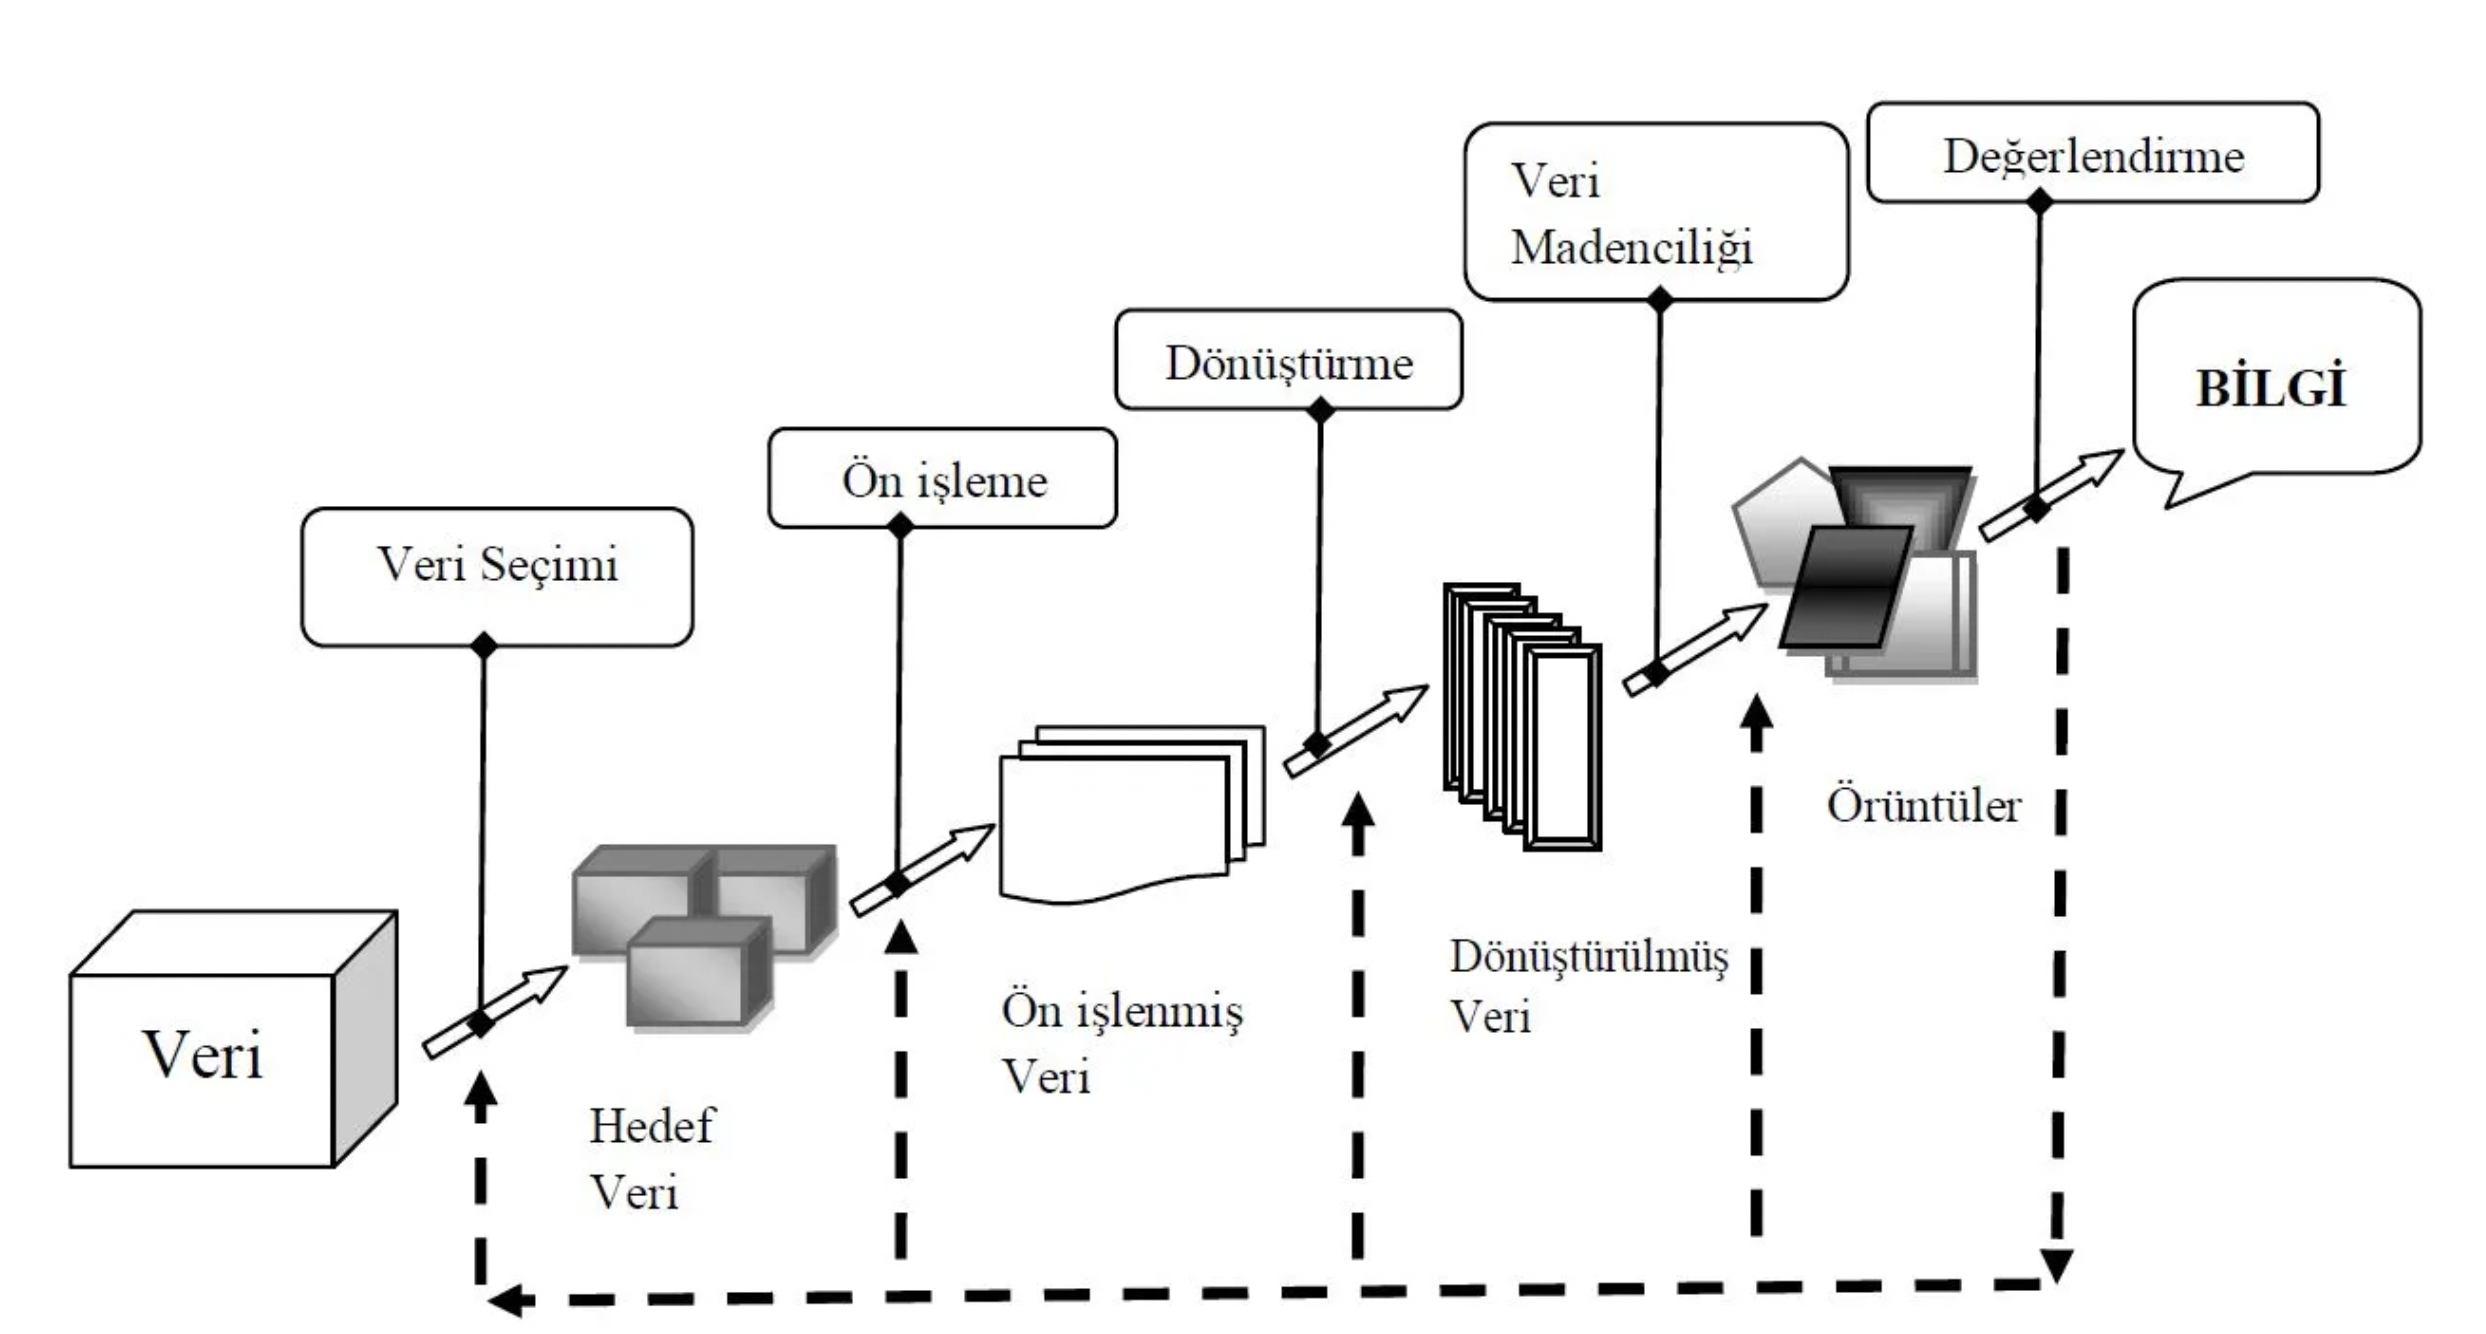
\includegraphics[width=11cm]{veri.png}
  \caption{Bilgi keşfi sürecinde veri madenciliği
 \cite{ref1}}
\end{figure}
\vspace{15pt}

\subsection{Bilginin Keşif Aşamaları}

\vspace{15pt}
\begin{itemize}
    \item Uygulama alanını inceleme 
    \item Amaca uygun veri kümesi oluşturma
    \item Veri ayıklama ve önişleme(işlemin \%70’lik bölümünü oluşturur)
    \item Veri azaltma ve veri dönüşümü (incelemede gerekli  özellikleri seçme, boyutlar arası ilişkiyi belirleme, boyut azaltma)
    \item Veri madenciliği tekniği seçme
    \item Sınıflandırma, eğri uydurma, bağıntı kuralları, demetleme
    \item Veri madenciliği algoritmasını seçme
    \item Model değerlendirme ve bilgi sunumu
    \item Bulunan bilginin yorumlanması
\end{itemize}

\begin{figure}[h]
\centering
  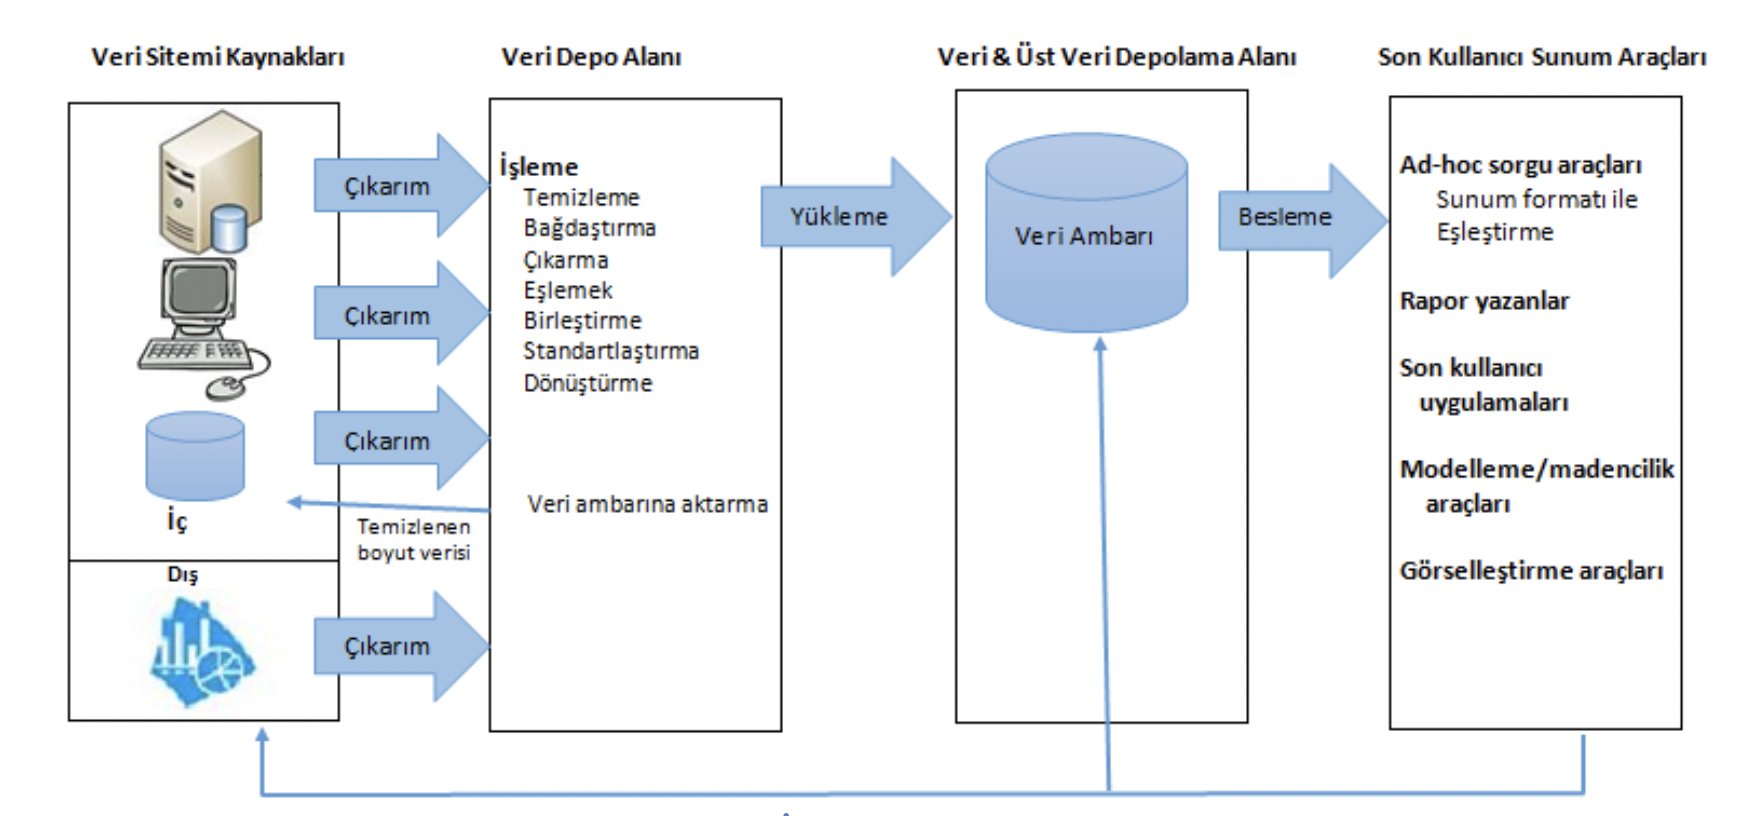
\includegraphics[width=15cm]{veriambar.png}
  \caption{İki Seviyeli Mimari
 \cite{ref2}}
\end{figure}

\newpage

\section{Veri Ambarı}
\vspace{10pt}
\subsection{Veri Ambarı Nedir?}

\vspace{10pt}
Veri ambarı kavramı, 1980'lerin sonlarına doğru ortaya çıkmış olup, ilk olarak IBM araştırmacıları Barry Devlin ve Paul Murphy tarafından bir iş veri ambarı (business datawarehouse) geliştirilmiştir. Barry Devlin tarafından yapılan tanıma göre, veri ambarı; farklı kaynaklardan toplanmış, son kullanıcının anlayabileceği ve ticari içeriklerde kullanabileceği hale getirilmiş, tek, tam ve tutarlı bir veri kaydıdır.

\vspace{10pt}
İş zekası analizi için gerekli veriyi sağlayan veri ambarı, iş zekasının önemli bir kaynağı olarak kabul edilmektedir. Veri ambarı, kuruluşların operasyonel veritabanı sistemlerindeki verileri analiz ve karar verme süreçlerine uygun bir şekilde düzenleyip sakladığı bir veri deposudur.

\vspace{5pt}
Veri ambarlarının kendine özgü birçok karakteristik özelliği vardır:
\vspace{5pt}

\begin{itemize}

    \item \textbf{Organize Edilmiş Veri: } Veri ambarı, farklı kaynaklardan gelen verileri düzenli bir şekilde depolar ve sunar.
    \item \textbf{Veride Tutarlılık: }Veri ambarı, tutarlı ve güvenilir veri sağlar, bu da doğru analiz ve kararlar almayı destekler.
    \item \textbf{Zamansal: }Veri ambarları, zaman içinde değişen verileri takip edebilme özelliğine sahiptir.
    \item \textbf{Kalıcı: }Veri ambarları, verileri kalıcı bir şekilde depolar ve uzun vadeli analiz ve raporlama için kullanılabilir.
    \item \textbf{İlişkisel Yapı: }Veri ambarları, ilişkisel veritabanı yapıları kullanarak verileri organize eder ve ilişkilendirir.
    \item \textbf{İstemci/Sunucu Mimarisi: }Veri ambarları, genellikle istemci/sunucu mimarisi üzerine kurulmuş sistemlerdir.
    \item \textbf{Web Tabanlı Destek: }Veri ambarları, kullanıcıların web tabanlı arayüzler üzerinden verilere erişmelerini sağlar.
    \item \textbf{Farklı Kaynaklar ile Entegrasyon: }Veri ambarları, çeşitli kaynaklardan gelen verileri entegre ederek bütünlük sağlar.
    \item \textbf{Gerçek Zamanlı Çalışma Yeteneği: }Veri ambarları, gerçek zamanlı çalışma yeteneği ile işletmelere anlık veri erişimi sağlar.
    
\end{itemize}

Bill Inmon  \cite{ref3} tarafından ortaya konan tanıma göre, veri ambarı; konu yönelimli, bütünleşmiş, zaman dilimli ve kalıcı veriler topluluğudur. Bu özellikler, veri ambarı sistemlerini diğer veritabanı sistemlerinden ayıran temel özelliklerdir.

\newpage

\subsection{Veri Ambarının Temel Özellikleri}

\vspace{10pt}
\textbf{Bütünleşik Yapı Sağlaması: }Veri ambarlarının temel özelliği, farklı veri kaynaklarından gelen verileri entegre bir ortamda tutabilmesidir. Bu entegrasyon, verilerin modellenerek tekrar eden bilgilerin temizlenmesiyle sağlanır. Böylece, karar vericiler ihtiyaç duydukları bilgilere tek bir sistem üzerinden erişebilirler. Bu bütünleşik yapı, veri analizlerini kolaylaştırarak karar alma süreçlerini optimize eder.

\vspace{10pt}
\textbf{Konu Odaklı Olması: }Veri ambarları, verileri konulara göre gruplandırarak tasnif eder. Kullanılmayacak veriler dışarıda tutularak basit ve özet bir bakış sağlanır. Veri ambarları, özellikle veri analizi için tasarlandığından, belirli konulara odaklanır. Örneğin, bir işletme müşteri konusuna odaklı bir veri ambarı inşa edebilir. Bu şekilde, işletme müşterileri hakkında daha fazla bilgi elde edebilir ve özel analizler yapabilir.

\vspace{10pt}
\textbf{Zaman Dilimli: }Veri ambarlarında veriler tarih bazlı olarak tutulur. Tüm veriler belirli bir zaman dilimine aittir. Bu yapı, zaman boyutunda karşılaştırmalar ve belirli bir zaman aralığına dayalı analizlerin yapılmasını mümkün kılar. Veri ambarı tasarımında genellikle tek bir zaman boyut tablosu oluşturularak bu ihtiyaçları karşılayabilecek zaman bilgileri içerilir.


\vspace{10pt}
\textbf{Kalıcı Veri Topluluğu: }Veri ambarında tutulan veri, kalıcı ve değiştirilemez bir yapıda olup, sık ekleme, güncelleme ve silme işlemlerine tabi değildir. Bu, operasyonel veritabanlarından farklıdır, çünkü temizlenmiş veri ambara aktarıldıktan sonra güncellenmez veya silinmez. Bu yapı, analizlerin tutarlılığı için kritiktir ve geçmişe yönelik veri analizlerinde tutarsızlıkların önüne geçer.

 \begin{figure}[h]
\centering
  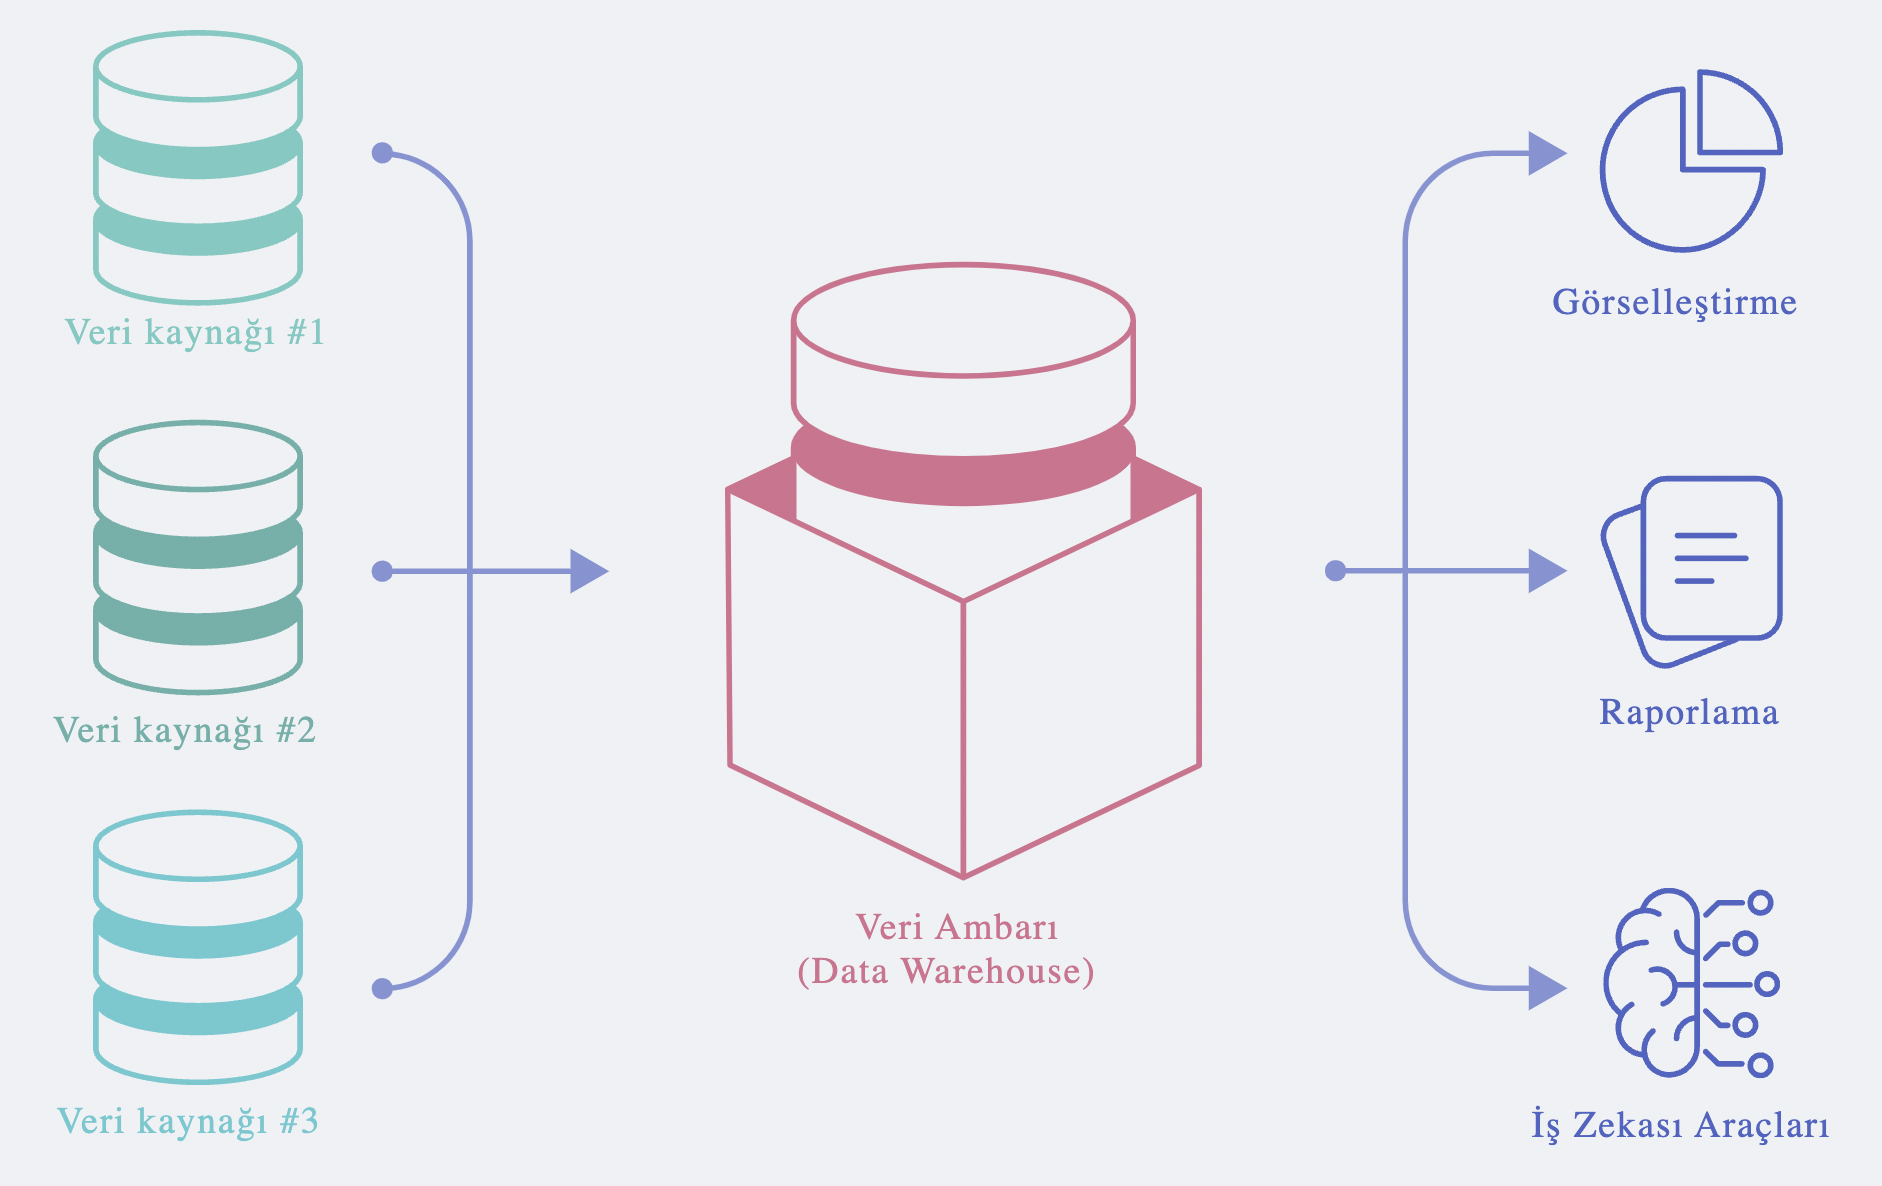
\includegraphics[width=10cm]{wirehouse.png}
  \caption{Data Warehouse\cite{ref4}}
\end{figure}

\newpage
\subsection{Veri Ambarı Mimarisi}
 
 Veri ambarı mimarisi konusunda, Bill Inmon ve Ralph Kimball arasında farklı yaklaşımlar bulunmaktadır. Inmon’un önerdiği tasarıma göre, ilk olarak bütünleşik ve geniş bir veri ambarı oluşturulmalıdır. Eğer data-mart ihtiyacı ortaya çıkarsa, bu ihtiyaç, zaten var olan bu ana veri ambarındaki verilerden karşılanmalıdır. Diğer taraftan, Kimball’ın önerdiği yöntemde ise, veri ambarı için data-mart’ların birleşimi başka bir şey değildir. İki farklı görüş, veri ambarı sistemlerine aşağıdan yukarıya (bottom-up) ve yukarıdan aşağıya (up-bottom) şeklinde iki temel yaklaşımı getirmiştir. Inmon’un normalize yaklaşımı, Kimball’ın boyutsal modelleme yaklaşımı olarak da adlandırılmaktadır.

\vspace{10pt}
 \textbf{1.Normalize Yaklaşım (Inmon Modeli)}

 Normalize yaklaşımına göre, veriler ilişkisel veri tabanlarında olduğu gibi normalizasyon kurallarına göre depolanır. Bu yaklaşımda, tarihsel boyutu olan, konu odaklı, kalıcı ve bütünleşmiş bir yapı kurularak tüm kurumsal veri burada depolanır. Amaç, verinin normalize bir formda değil, her verinin tek bir erişim noktasının olmasıyla veri entegrasyonunu sağlamaktır. Veri entegrasyonu, farklı kaynaklardan alınan verinin tek bir ortamda aynı veri deseni altında toplanması ve erişilmek istenen bilginin tek bir adresinin olmasıdır.

 Normalize yaklaşımıyla oluşturulan veri ambarlarında, verilerin normalize ve atomik yapısı nedeniyle veri çekmek zordur. Bu yapı, büyük kurumsal yapıların uygulandığında, birbirleriyle bağlantılı yüzlerce tablodan oluşan bir ağ yapısı oluşturur. Bu yaklaşımın faydası, her yeni verinin basit bir şekilde veritabanına eklenmesidir, ancak her yeni veriyle veritabanındaki tablo sayısı da artar. Bu nedenle, farklı kaynaklardan veri alındığında çok fazla tablo bağlantısı kurulması ve bilgiye erişimde zorluk yaşanabilir. Bu zorlukları aşmak için, veri ambarını kaynak olarak kullanan ve datamart’ları bölümsel alt kümeler olarak tanımlayan bir yöntem kullanılır. Kullanıcılar, oluşturulan datamart’lar üzerinden sorgularını çeker ve analizlerini yaparlar. Bu mimariye “hub-and-spoke” mimarisi denir. 
 \begin{figure}[h]
\centering
  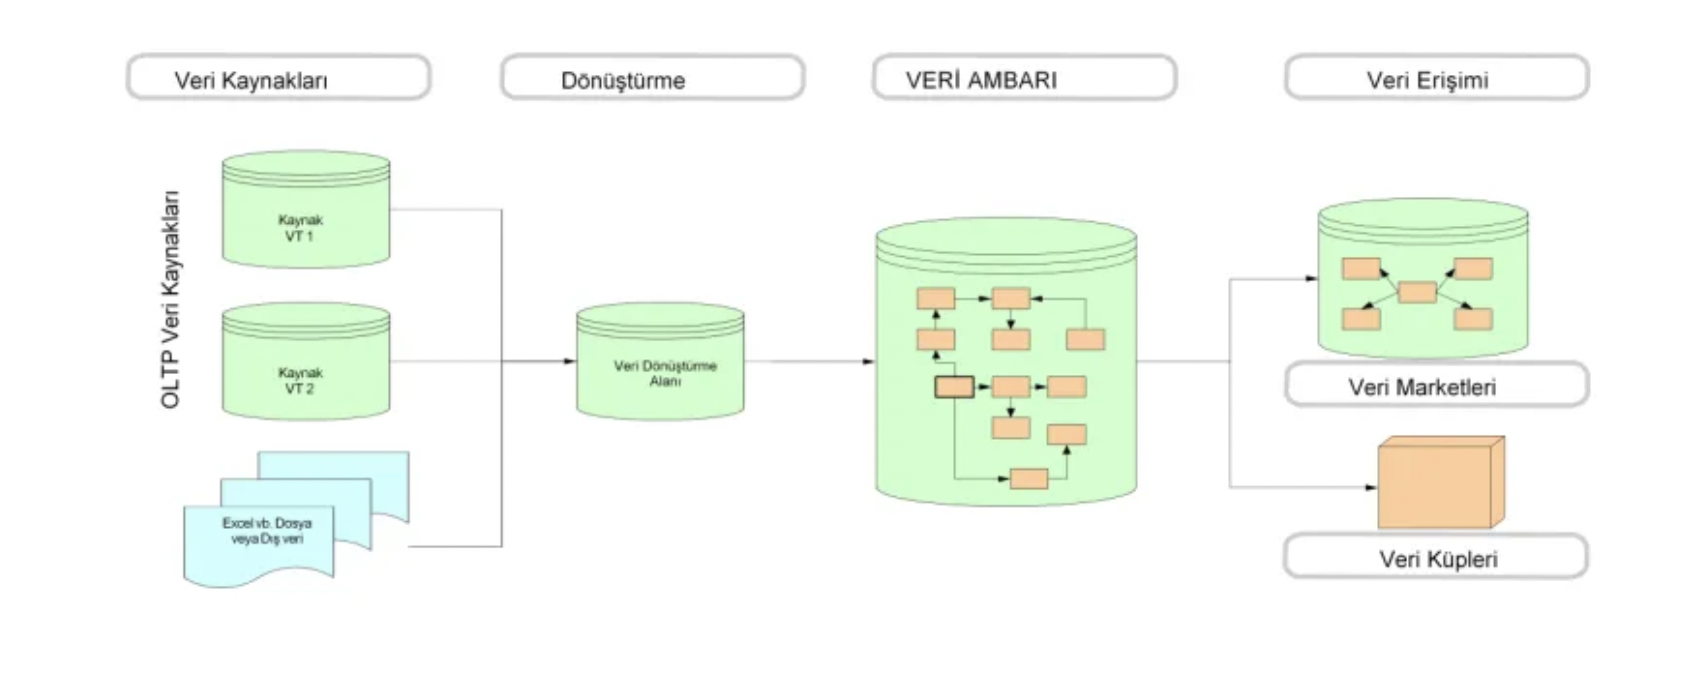
\includegraphics[width=11cm]{norm.png}
  \caption{Inmon Modeli\cite{ref5}}
\end{figure}
\newpage
\textbf{2.Boyutsal modelleme (Kimball modeli)}

Ralph Kimball’ın geliştirdiği boyutsal modelleme veya Yıldız Şema olarak bilinen yöntem, aşağıdan yukarıya odaklanan bir veri ambarı mimarisidir. Kimball’ın boyutsal yaklaşımı, tasarım sürecine odaklanan bir mimariye sahiptir. Bu modelde, merkezi bir yapıda ortak bir desen oluşturmak yerine, doğrudan departman veya konu odaklı datamart’lar oluşturulur ve bu datamart’lar kullanıcıların erişimine açılır. Veri ambarı, bu datamart’ların birleşiminden oluşur.

Boyutsal modelleme yönteminde, veri ambarı merkezi bir veri ambarından türetilmez; bunun yerine, datamart’lar üzerinden oluşturulur. Bu yaklaşım, normalize yaklaşımdan farklı olarak daha dağıtık bir yapı sunar. Şekilde gösterildiği gibi, veri ambarı, farklı datamart’ların birleşiminden meydana gelir.

 \begin{figure}[h]
\centering
  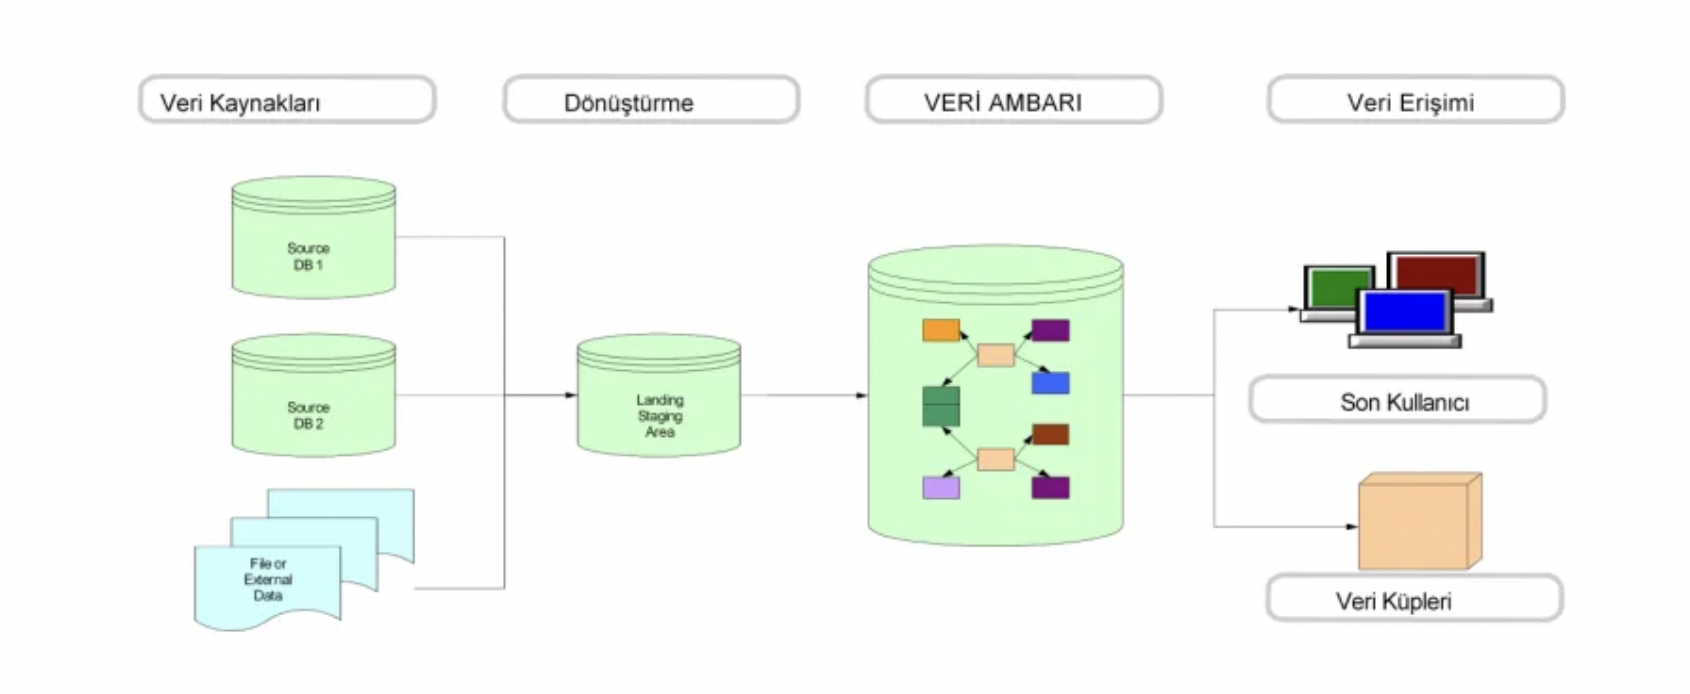
\includegraphics[width=13cm]{kimbal.png}
  \caption{Kimball modeli\cite{ref6}}
\end{figure}

\section{Veri Madenciliğindeki Problemler}
\vspace{10pt}
Veri madenciliği girdi olarak ham veriyi sağlamak üzere veri tabanlarına
dayanır. Bu da veri tabanlarının dinamik, eksiksiz, geniş ve net veri içermemesi
durumunda sorunlar doğurur. Diğer sorunlar da verinin konu ile uyumsuzluğundan
doğabilir.
Sınıflandırmak gerekirse başlıca sorunlar şunlardır :
\vspace{10pt}
\begin{itemize}
    
    \item \textbf{Sınırlı Bilgi : }Veri tabanları genel olarak veri madenciliği dışındaki
amaçlar için tasarlanmışlardır. Bu yüzden, öğrenme görevini
kolaylaştıracak bazı özellikler bulunmayabilir.
    \item \textbf{Gürültü ve Eksik Değerler : }Veriözellikleri ya da sınıflarındaki
hatalara gürültü adı verilir. Veri tabanlarındaki eksik bilgi ve bu yanlışlardan dolayı veri madenciliği amacına tam olarak ulaşmayabilir. Bu bilgi yanlışlığı, ölçüm hatalarından, ya da öznel yaklaşımdan
olabilir
    \item \textbf{Belirsizlik : }Yanlışlıkların şiddeti ve verideki gürültünün derecesi ile
ilgilidir. Veri tahmini bir keşif sisteminde önemli bir husustur. 
    \item \textbf{Ebat, güncellemeler ve konu dışı sahalar :} Veri tabanlarındaki bilgiler,
veri eklendikçe ya da silindikçe değişebilir. Veri madenciliği
perspektifinden bakıldığında, kuralların hala aynı kalıp kalmadığı ve
istikrarlılığı problemi ortaya çıkar. Öğrenme sistemi, kimi verilerin
zamanla değişmesine ve keşif sisteminin verinin zamansızlığına karşın
zaman duyarlı olmalıdır. 
\end{itemize}

\vspace{10pt}
\section{Sonuç}

Yeni nesil internet, yaklaşık 155 Mbits/sn lik hatta belki de daha da
üzerinde hızları kullanmamızı sağlayacak. Bu da günümüzde kullanılan bilgisayar
ağlarındaki hızın 100 katından daha fazla bir sürat ve taşıma kapasitesi demektir.
Böyle bir bilgisayar ağı ortamı oluştuktan sonra, dağıtık verileri analiz etmek ve
farklı algoritmaları kullanmak mümkün olacaktır. Bundan 10 yıl önceki bilgisayar
ağları teknolojisinde hayal edemediklerimizi artık kullanabiliyoruz. Buna bağlı
olarak, veri madenciliğine uygun ağların tasarımı da yapılmaktadır. Veri
madenciliği, sayısal ve istatistiksel olarak büyük veri kümeleri üzerinde yoğun
işlemler yapmayı gerektirir. Gelişen bellek ve işlem hızı kapasitesi sayesinde,
birkaç yıl önce madencilik yapılamayan veriler üzerinde çalışmayı mümkün hale
getirmiştir. Günümüzde ticaret ve işler çok karlı olmalı, daha hızlı ilerlemeli ve
daha yüksek kalitede servis ve hizmet verme yönünde olmalı, bütün bunları
yaparken de minimum maliyeti ve en az insan gücünü göz önünde
bulundurmalıdır. Bu tip hedef ve kısıtların yer aldığı iş dünyasında veri
madenciliği, temel teknolojilerden biri haline gelmiştir. Çünkü veri madenciliği sayesinde müşterilerin ve müşteri faaliyetlerinin yarattığı fırsatlar daha kolay
tespit edilebilmekte ve riskler daha açık görülebilmektedir.

\vspace{15pt}
\begin{thebibliography}
    .\bibitem{ref1} \href {https://tr.linkedin.com/pulse/crisp-dm}{https://tr.linkedin.com/pulse/crisp-dm}

    \bibitem{ref2} \href {https://medium.com/cem.yldrm9901/veri-ambari-modelleme}{https://medium.com/cem.yldrm9901/veri-ambari-modelleme}

    \bibitem{ref3} \href {https://www.astera.com/type/blog/data-warehouse-concepts/}{https://www.astera.com/type/blog/data-warehouse-concepts/}

    \bibitem{ref4} \href {https://www.estebilisim.com/data-warehouse-cloud-on-premise/}{https://www.estebilisim.com/data-warehouse-cloud-on-premise/}

    \bibitem{ref5} \href {https://link.springer.com/chapter/10.1007/978-981-16-7610-9_57}{https://link.springer.com/chapter/10.1007/978-981-16-7610-9_57}

    \bibitem{ref6} \href {https://www.existbi.com/blog/informatica-training-best-practices/}{https://www.existbi.com/blog/informatica-training-best-practices/}
    

\end{thebibliography}

\end{document}
